\subsubsection{\label{database} Database}

Dieses Paket\ref{fig:database_package}  kontrolliert alle Daten die in die Datenbank geschrieben werden.
Entweder sollen Daten in die Datenbank geschrieben werden, oder sie sollen ausgelesen werden. Die Antwort ist dementsprechend entweder leer, die gewünschten Daten, oder, im Fall von Unstimmigkeiten, eine Fehlermeldung.

Da jede Klasse auf dem Singleton Entwurfsmuster aufbaut wurden sämtliche darauf basierenden Parameter und Funktionen weggelassen.


\class{WorkflowData}
Diese Klasse ist die Schnittstelle für alle Klassen die auf den Datenbankeinträgen für Workflows arbeiten wollen. Sie erstellt für jeden Zugriff den passenden Datenbankbefehl und konvertiert die Ergebnisse in das gewünschte Format des Aufrufers.
Sie wirft bei fehlerhaften Werten eine entsprechende \textbf{MatFlowException}.

Diese Klasse, sowie alle anderen im Paket Database, ist nach dem Singleton Entwurfsmuster entworfen, da so Aufträge an die Datenbank so zentriert gesendet werden können.
\begin{figure}[h]
	\centering
	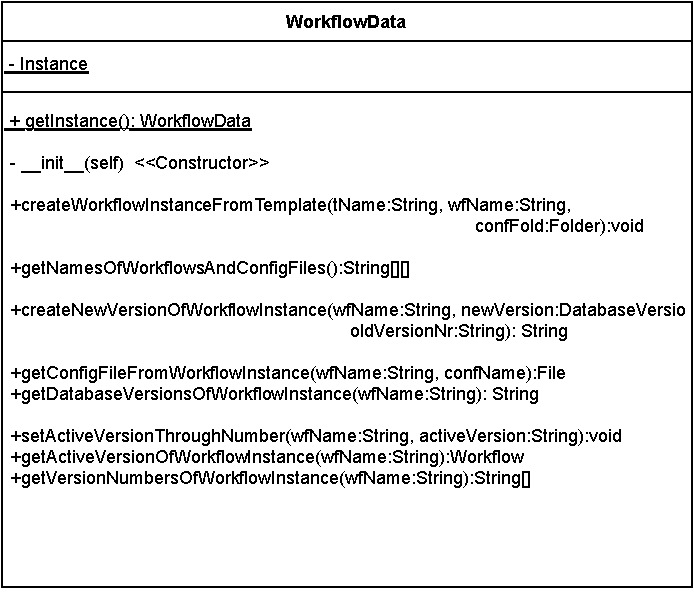
\includegraphics[width=0.7\textwidth]{res/Klassen/WorkflowData.pdf} 
	\caption{WorkflowData}
	\label{fig:workflowDataClass}
\end{figure}

\begin{methodenv}{Methods}

\method{createWorkflowInstanceFromTemplate(tName: String, wfName: String, confFold: Folder):void}
Create a new instance of a workflow by using the dag-file of a Template, 
with the Version set to 1. 
Search confDirect for every .conf-file and add them into the Database.
Set this Version as active Version.

\smallPara{Parameters}
\begin{itemize}
	\item tName
	name of Template of which the dag should be taken from
	\item wfName
	name of the new Workflow
	\item confFold
	the folder where all data of the Workflow is saved into
\end{itemize}


\method{getNamesOfWorkflowsAndConfigFiles():String[][]]}
Return all Workflow names and the names of their corresponding config files.
The returning value is a list of lists of Strings where an inner list has the form [<Workflow Name>, <config File1 Name>, <config File2 Name>, ...]

\method{createNewVersionOfWorkflowInstance(wfName:String, newVersion:DatabaseVersion, oldVersionNr:String):void}
Create a new Version of an existing Workflow with changed config Files.
Search which config Files changed and set those in the new Version.

\smallPara{Parameters}
\begin{itemize}
	\item \textbf{wfName}
	name of the Workflow
	\item \textbf{newVerson}
	new Version identifier
	\item \textbf{oldVersionNr}
	identifier of Version the new one is based on
\end{itemize}

\method{getDatabaseVersionsOfWorkflowInstance(wfName:String):DatabaseVersion[]}
 Return all Versions of a Workflow Instance as DatabaseVersion Objects in a list.
 Asks the Database for the data and constructs every Object.
 
 \smallPara{Parameters}
\begin{itemize}
	\item \textbf{wfName}
	name of the Workflow
\end{itemize}

\method{setActiveVersionThroughNumber(wfName:String, version:String):void}
Set the previous Version as inactive and a new Version as active

\smallPara{Parameters}
\begin{itemize}
	\item \textbf{wfName}
	name of the Workflow
	\item \textbf{version}
	version to be set active
\end{itemize}

\method{getVersionNumbersOfWorkflowInstance(wfName:String):String[]}
Return a sortet list of Strings of all Versions of a Workflow.

\smallPara{Parameters}
\begin{itemize}
	\item \textbf{wfName}
	name of Workflow which versions should be listed
\end{itemize}

\end{methodenv}

%%%%%%%%%%%%%%%%%%%%%%%%%%%%%%%%%%%%%%%%%%%%%%%%%%%%%%%%%%%%%

\subsubsection{TemplateData}
Diese Klasse ist die Schnittstelle für alle Klassen die auf den Datenbankeinträgen für Workflow\_Template arbeiten wollen. Sie erstellt für jeden Zugriff den passenden Datenbankbefehl und konvertiert die Ergebnisse in das gewünschte Format des Aufrufers.
Sie wirft bei fehlerhaften Werten eine entsprechende \textbf{MatFlowException}.

Diese Klasse, sowie alle anderen im Paket Database, ist nach dem Singleton Entwurfsmuster entworfen, da so Aufträge an die Datenbank so zentriert gesendet werden können.
\begin{figure}[h]
	\centering
	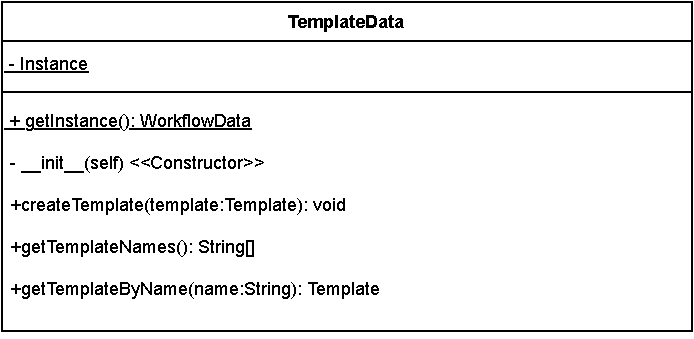
\includegraphics[width=0.7\textwidth]{res/Klassen/TemplateData.pdf} 
	\caption{WorkflowData}
	\label{fig:workflowDataClass}
\end{figure}

\begin{methodenv}{Methods}
	
\method{createTemplate(template:Template):void}
Read Values from template and convert them into a sql query.
Throw error if name already exists.

\smallPara{Parameters}
\begin{itemize}
	\item \textbf{template}
	Template object to convert
\end{itemize}

\method{getTemplateNames():String[]}
Return a list of all existing Template names.
List is empty when no Template exists.

\method{getTemplateByNames(name:String):Template}
Return Template that is asked for.
Throw error if Template doesn't exist.

\smallPara{Parameters}
\begin{itemize}
	\item \textbf{name}
	name/identifier of the wanted Template
\end{itemize}

\end{methodenv}
%%%%%%%%%%%%%%%%%%%%%%%%%%%%%%%%%%%%%%%%%%%%%%%%%%%%%%%%%%%%%%%%%%

\subsubsection{ServerData}
Diese Klasse ist die Schnittstelle für alle Klassen die auf den Datenbankeintrag für Server arbeiten wollen. Sie erstellt für jeden Zugriff den passenden Datenbankbefehl und konvertiert die Ergebnisse in das gewünschte Format des Aufrufers.
Sie wirft bei fehlerhaften Werten eine entsprechende \textbf{MatFlowException}.

Diese Klasse, sowie alle anderen im Paket Database, ist nach dem Singleton Entwurfsmuster entworfen, da so Aufträge an die Datenbank so zentriert gesendet werden können.
\begin{figure}[h]
	\centering
	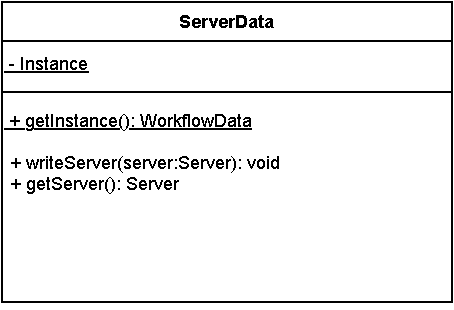
\includegraphics[width=0.7\textwidth]{res/Klassen/ServerData.pdf} 
	\caption{WorkflowData}
	\label{fig:workflowDataClass}
\end{figure}

\begin{methodenv}{Methods}
	
\method{set(create: String):String} Create new entry on Database. Try to execute create on Database and return value.

\smallPara{Parameters}
\begin{itemize}
	\item \textbf{create} 
	a sql query to create an entry
\end{itemize}

\method{delete(del: String):String} Delete an existing entry. Try to execute del on Database and return value.

\smallPara{Parameters}
\begin{itemize}
	\item \textbf{del} 
	a sql query to delete an entry
\end{itemize}

\method{modify(change: String):String} Modify an existing entry. Try to execute change on Database and return value.

\smallPara{Parameters}
\begin{itemize}
	\item \textbf{change} 
	a sql query to change values
\end{itemize}

\end{methodenv}
%%%%%%%%%%%%%%%%%%%%%%%%%%%%%%%%%%%%%%%%%%%%%%%%%%%%%%%%%%%%%%%%%%

\subsubsection{DatabaseTable}
DatabaseTable ist die einzige Klasse die direkt mit der Datenbank kommuniziert. Ihre Funktion ist hauptsächlich MySQL Befehle entgegennimmt, diese an die Datenbank weiterzugeben und die dadurch erhaltenen Antworten zurückgibt. Im Fall eines Fehlers, wie einem leeren Ergebnis oder eines ungültigen Befehls wird eine entsprechende \textbf{MatFlowException} geworfen.

Diese Klasse, sowie alle anderen im Paket Database, ist nach dem Singleton Entwurfsmuster entworfen, da so Aufträge an die Datenbank so zentriert gesendet werden können.
\begin{figure}[h]
	\centering
	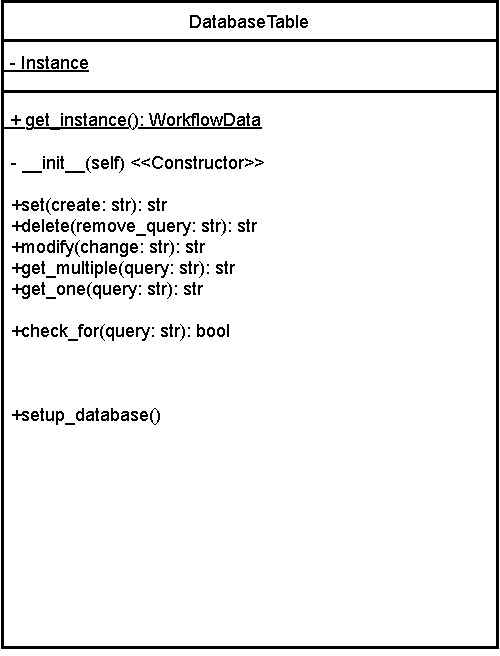
\includegraphics[width=0.7\textwidth]{res/Klassen/DatabaseTable.pdf} 
	\caption{WorkflowData}
	\label{fig:workflowDataClass}
\end{figure}

\begin{methodenv}{Methods}
	
	\method{set(create: String):String} Create new entry on Database. Try to execute create on Database and return value.
	
	\smallPara{Parameters}
	\begin{itemize}
		\item \textbf{create} 
		a sql query to create an entry
	\end{itemize}
	
	\method{delete(del: String):String} Delete an existing entry. Try to execute del on Database and return value.
	
	\smallPara{Parameters}
	\begin{itemize}
		\item \textbf{del} 
		a sql query to delete an entry
	\end{itemize}
	
	\method{modify(change: String):String} Modify an existing entry. Try to execute change on Database and return value.
	
	\smallPara{Parameters}
	\begin{itemize}
		\item \textbf{change} 
		a sql query to change values
	\end{itemize}

	\method{get(query: String):String} Try to get a specific value, or values and returnit.

	\smallPara{Parameters}
	\begin{itemize}
		\item \textbf{query} 
		a sql query to get information
	\end{itemize}
	
\end{methodenv}

\newpage